\section{Validation with Data from Photon Detector System Prototypes}
\label{sec:dp-pds-prototypes}

\subsection{Design Similarities and Differences Between Prototypes and Far Detector System}
The \dword{lar} \dword{tpc} \dword{dp} proposed technology is the result of years of R\&D. From small-scale chambers to the \dword{dune} module, many prototypes have been constructed, each with some design modifications and optimizations. 
Relevant to the \dword{pds} itself, the \dword{wa105}, operated at CERN in 2017, the \dword{pddp}, to be commissioned in 2019 and the \dword{dune} far detector module similarities and differences will be described here.

The first tonne scale dual phase \dword{lar} \dword{tpc} demonstrator has taken cosmic data between June and November \num{2017} at CERN. 
Located \SI{1}{m} below the charge collection plane, underneath the cathode and the \dword{gg}, the photon detection system consisted of five \dwords{pmt} (Hamamatsu R5912-MOD20, described in more detail in Sec.~\ref{sec:dp-pds-selection-procurement}) evenly distributed along the 3$\times$1~m$^2$ area (one \dword{pmt} every \SI{50}{cm}). The demonstrator was considered as an opportunity to test different \dword{pds} designs, in particular in terms of \dword{tpb} coating and front-end electronics. Three \dwords{pmt} had the \dword{tpb} coating applied with evaporation directly onto their windows, whereas for the other two, the \dword{tpb} was deposited on a \SI{4}{\mm} thick transparent Plexiglass plate which was mounted on top of the \dwords{pmt}. 
While the latter solution has the advantage of being simpler and less risky to manipulate, it reduces the acceptance and possibly the efficiency due to the internal reflections between the \dword{tpb} and the Plexiglass surfaces. 
Pictures of the \dword{wa105} \dword{pds} are shown in Figure~\ref{fig:pd-pds-311-pmt-tpb}.

\begin{dunefigure}[\dword{wa105} \dword{pds} ]{fig:pd-pds-311-pmt-tpb}{The \dword{wa105} \dword{pds}. Top left: \dword{pmt} with the \dword{tpb} deposited on the plexiglass plate, top right: \dword{pmt} with the \dword{tpb} coated onto the photocathode. Bottom: The five \dwords{pmt} installed in the \dword{wa105}, underneath the ground grid.}
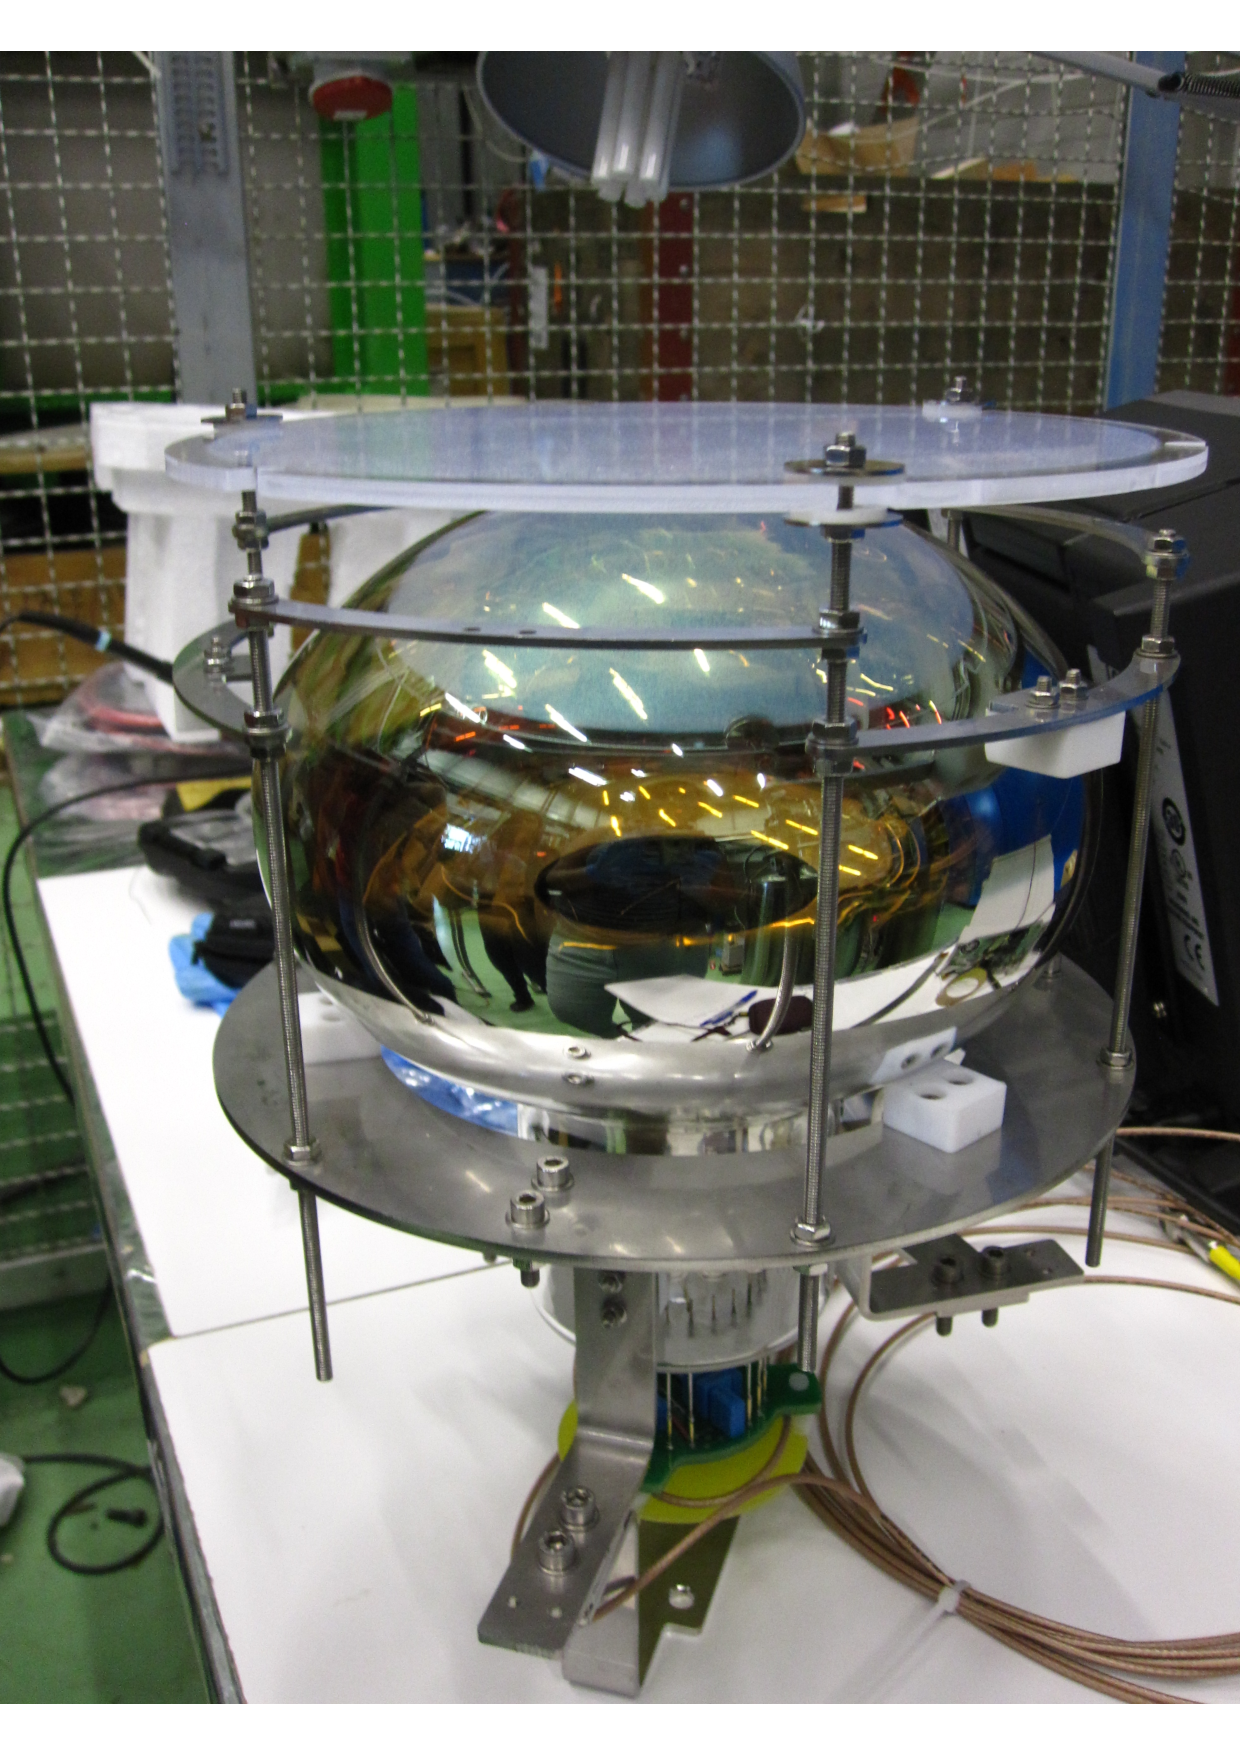
\includegraphics[width=0.25\textwidth]{graphics/dppd_PMTPlate}
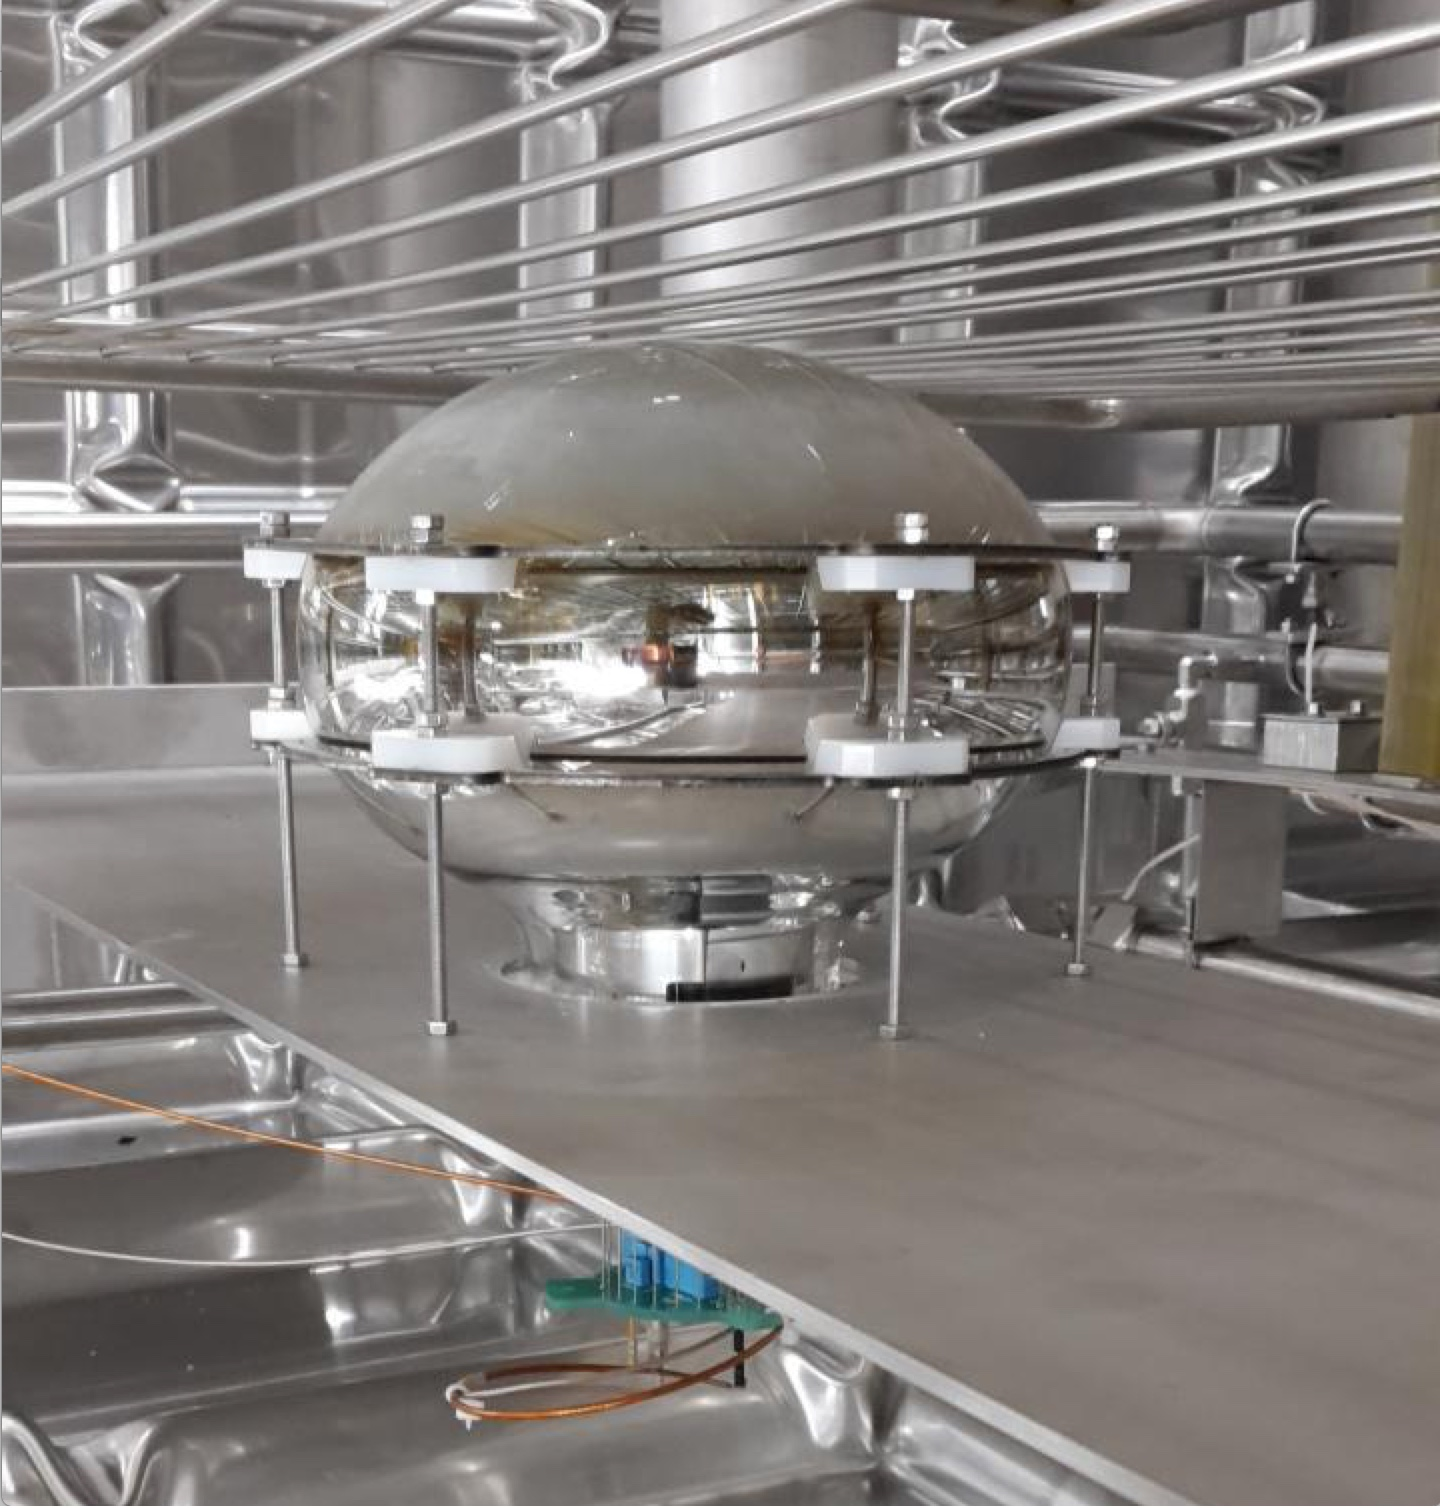
\includegraphics[width=0.33\textwidth]{graphics/dppd_PMTTPB.jpeg}\\
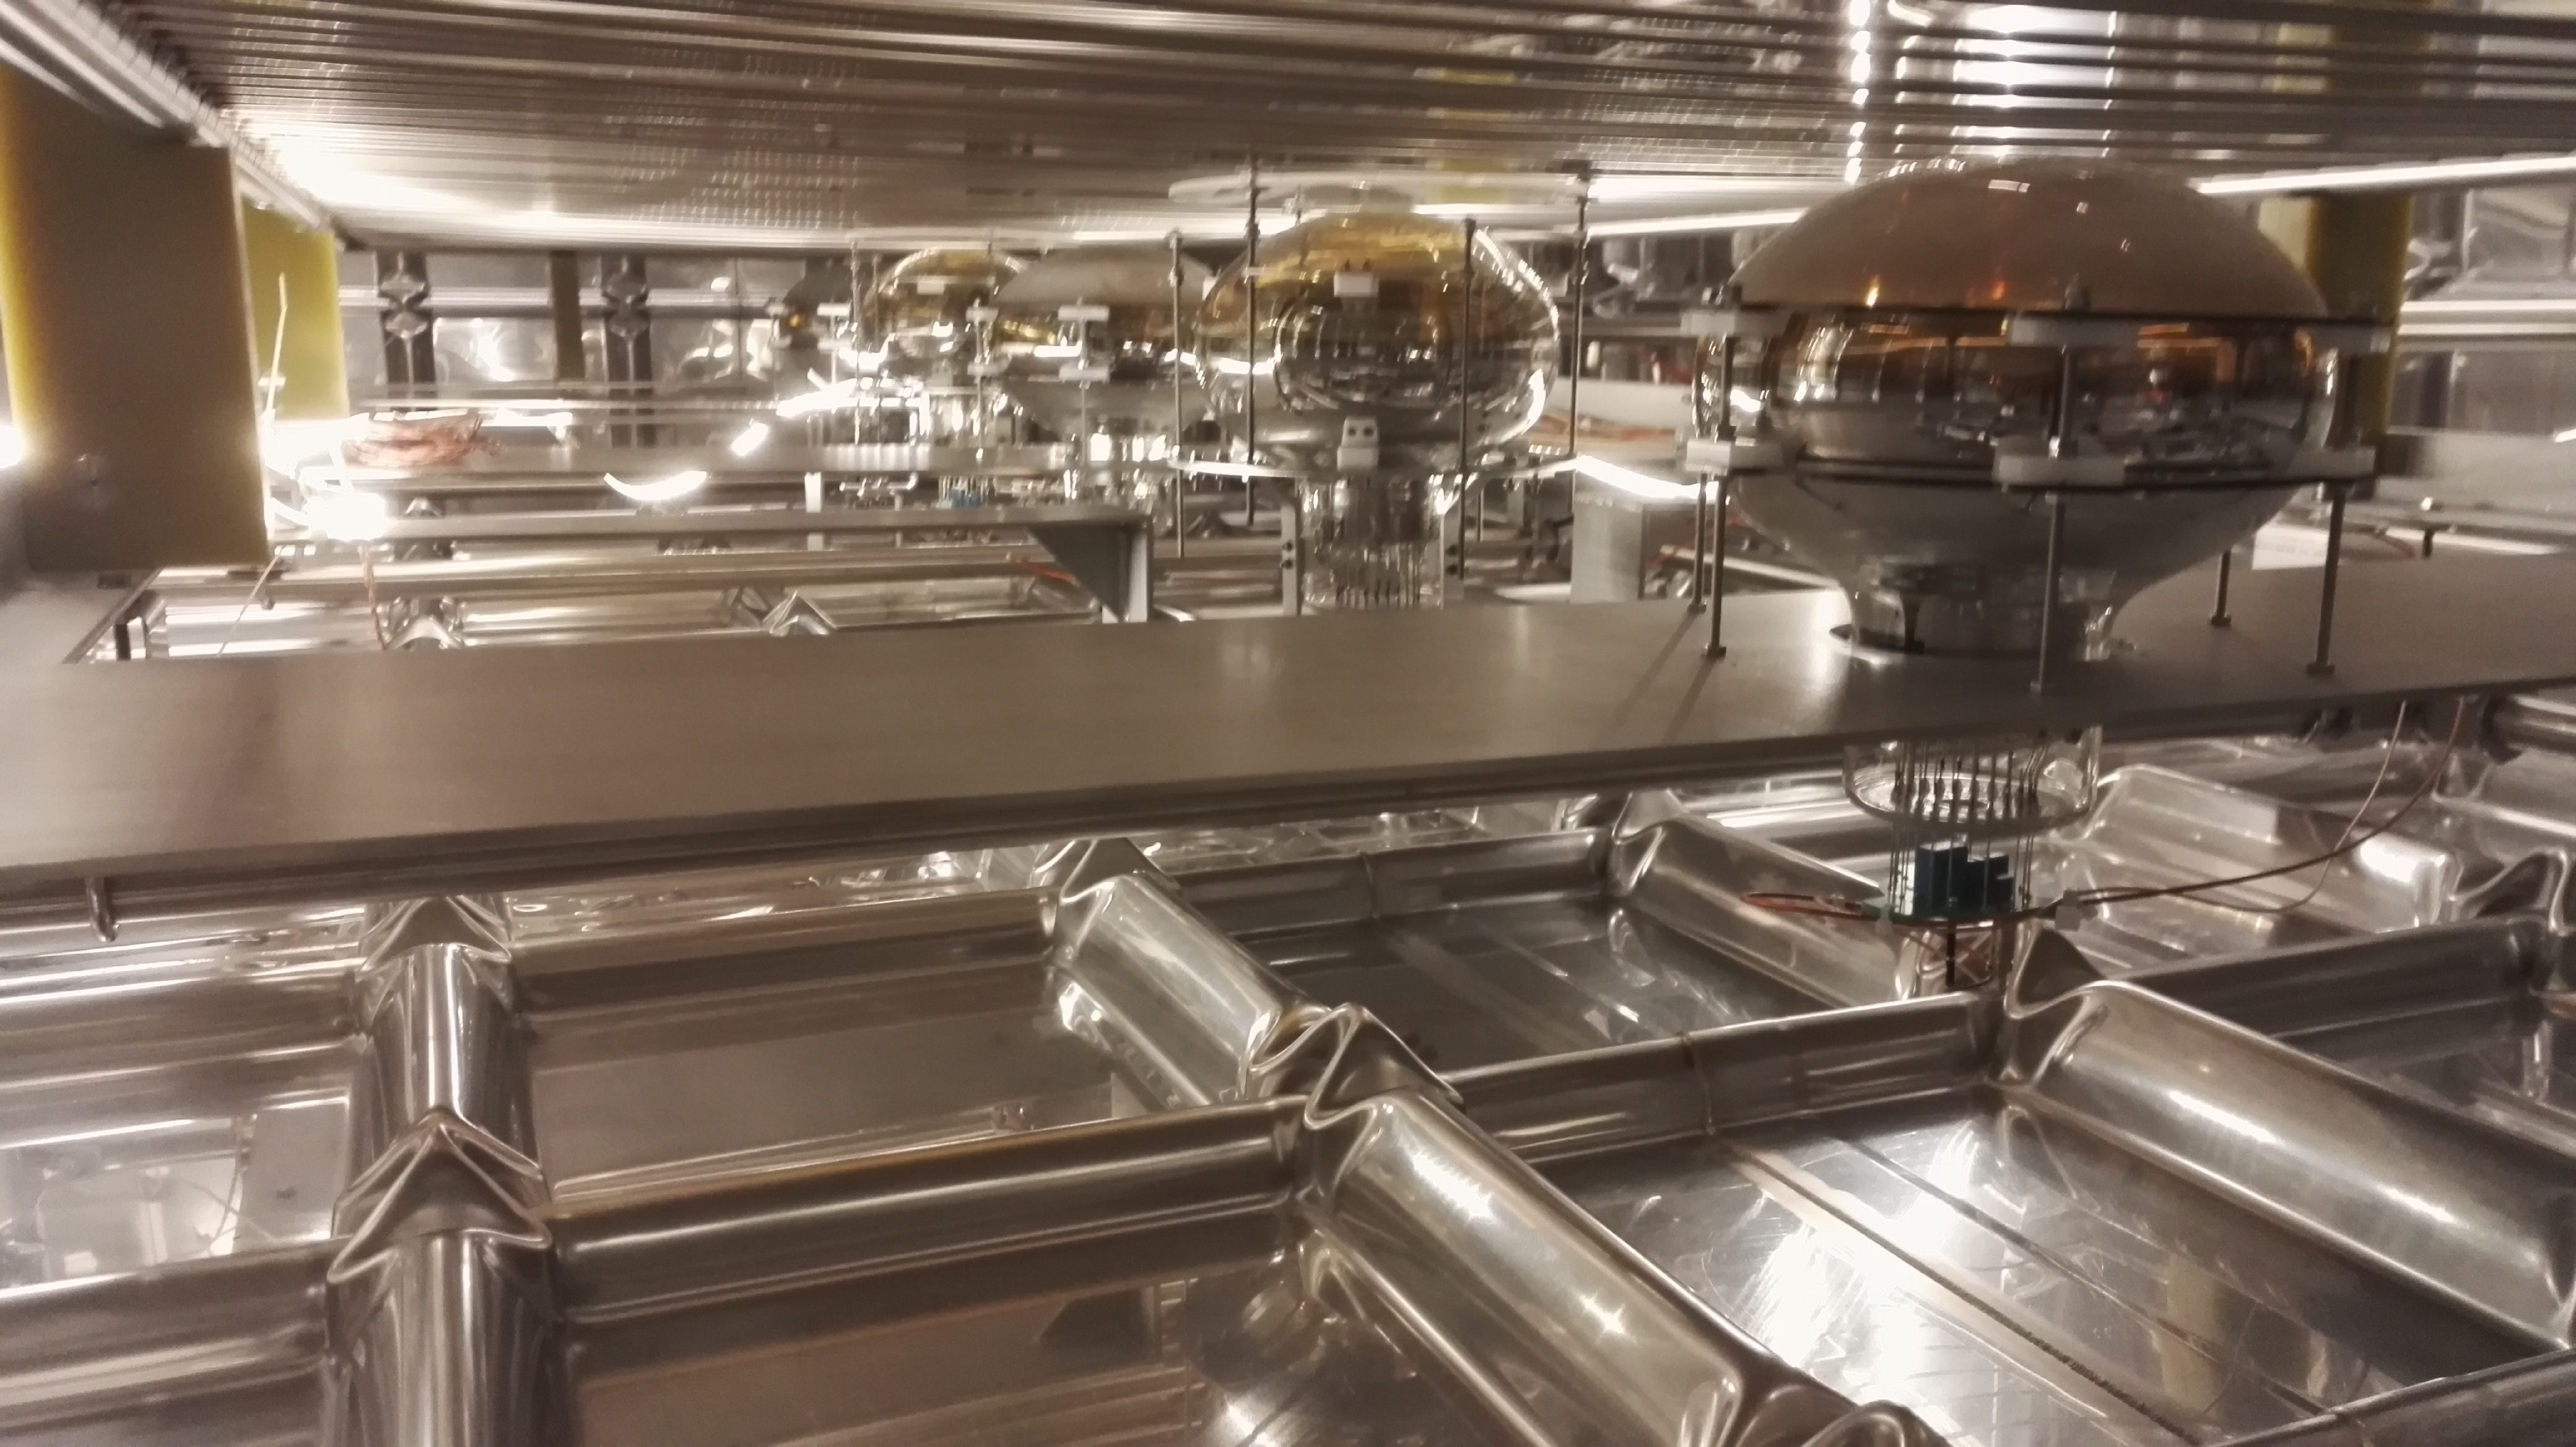
\includegraphics[width=0.6\textwidth]{graphics/dppd_PMT_311_installation.jpg}
\end{dunefigure}

Two power supply polarities were used. Three \dwords{pmt} were equipped with a negative \dword{hv} base, i.e. a negative bias voltage is applied to the photocathode and the anode is grounded. This system requires two cables: one for the \dword{hv} system and one for the signal. A positive base was serving the other two \dwords{pmt}: a single cable positively biases the anode and carries the signal, and the cathode is grounded. The \dword{hv} and the signal are then externally decoupled using a splitter, see Sec.~\ref{sec:fddp-pd-4.2}. The latter design has the advantage of reducing the number of feedthroughs and cables while also reducing the noise. Overall, four configurations were tested, as presented in Table~\ref{tab:dp-pds-311conf}. During the 3$\times$1$\times$1~m$^3$ operation, the \dwords{pmt} were operated at a rather uniform gain of around \num{e6} with a readout sampling of \SI{250}{MHz}.

\begin{dunetable}
[\dword{wa105} \dwords{pmt} configurations.]
{cccccc}
{tab:dp-pds-311conf}
{Configuration of the five \dwords{pmt} installed in the \dword{wa105}}
\dword{pmt} & Base & Coating & Voltage (kV) & Gain (\num{e6}) & Noise (ADC)\\
%\hline
1 & Negative & Coating & \num{-1.2} & 0.92$\pm$0.13 & \num{0.7} \\
2 & Negative & Plate   & \num{-1.2} & 1.01$\pm$0.12 & \num{0.7} \\
3 & Positive & Coating & \num{1.1} & 0.95$\pm$0.11 & \num{0.4} \\
4 & Positive & Plate   & \num{1.1} & 1.26$\pm$0.15 & \num{0.4} \\
5 & Negative & Coating & \num{-1.2} & 1.33$\pm$0.15 & \num{0.8} \\
%\hline
\end{dunetable}

In \dword{pddp}, \num{36} \dwords{pmt} are installed \SI{6}{\m} below the collection plane, again underneath the cathode and the \dword{gg}. The \dword{pmt} density is lower compared to the demonstrator. Their positioning over the \SI{36}{m$^2$} area was optimized with simulations. The number of \dwords{pmt} is higher around the center of the active volume and lower near the \dword{fc} borders. This positioning maximizes the amount of light collection from cosmic rays.

Following the evaluation of the demonstrator configurations, the \dword{tpb} was directly evaporated onto the \dword{pmt} windows and the electronic base was chosen to have positive polarity. This configuration maximizes the collection efficiency, and reduces both the number of cables and the electronic noise. 

For \dword{dune} \dword{fd} \dword{pds}, \dword{tpb} will be directly coated onto the \dword{pmt} windows and positive biasing scheme will be implemented. As the aspect ratio between cathode size and drift distance is larger compared to \dword{pddp}, the amount of light loss by absorption on the \dword{fc} is expected to be smaller. Therefore, the \dword{dune} \dword{fd} \dword{pds} layout is foreseen to be uniform, with \dwords{pmt} on a regular lattice with \SI{1.02}{m} spacing. On the other hand, light attenuation due to absorption in the \lar itself will be larger in the \dune \dpmod.

%%%%%%%%%%%%%%%%%%%%%%%%%%%%%%%%%%%%%%%%%%%%%%%%%%%%%%%%%%%%%%%%%%%%

\subsection{\dword{wa105} Light Data Results and Simulation Validation}

\fixme{The \dword{wa105} simulation to be validated in this section needs to change from LightSim to \dword{larsoft}}

The analysis of the data taken during the \dword{wa105} operation provides the first handle on the validation and improvement of the light simulation developed so far. 
The active volume of the demonstrator ($3\times1\times1$~m$^3$) is rather small with respect to the Rayleigh scattering length, which is of the order of \SI{60}{\cm}. 
As a consequence, the light absorbed by elements of the detector (such as the \dword{fc}, \dword{lem} or cathode) may become a dominant factor.
Hence, the light maps were created with particular care given to the precision in the reproduction of the demonstrator's geometry.

Two triggering schemes were used during the \dword{wa105} operation.
The first was provided by an external muon tagger, the Cosmic Ray Tagger (CRT), to record horizontal muons. The CRT was made of plastic scintillator planes located on each side of the detector.
The second was performed by the \dwords{pmt} themselves, requiring that the five sensors recorded sufficient amount of light in coincidence. In this configuration, a higher number of vertical muons were recorded, as well as showers.

In the CRT trigger condition, a rough track reconstruction is possible as the CRT provides coordinate information with \SI{11}{\cm$^2$} resolution. Hence, even without the charge information, like for data taken at null field, it is possible to select muon-like tracks and to retrieve the shortest distance between the track and each \dword{pmt}. A schematic drawing of the \dword{wa105} detector is presented in Fig.~\ref{fig:pd-pds-311schema}, along with the relevant track parameters.

\begin{dunefigure}[\dword{wa105} schematic drawing]{fig:pd-pds-311schema}{Schematic view of the \dword{wa105}. 
The fiducial volume is represented in gray and is limited from the collection plane area to the cathode. In yellow, the active volume is presented. Its volume is defined by the collection plane, the \dword{fc} to the top of the \dwords{pmt}. A track that would be detected by the CRTs is shown, with its minimum distance to \dword{pmt} \num{3} shown in red.}
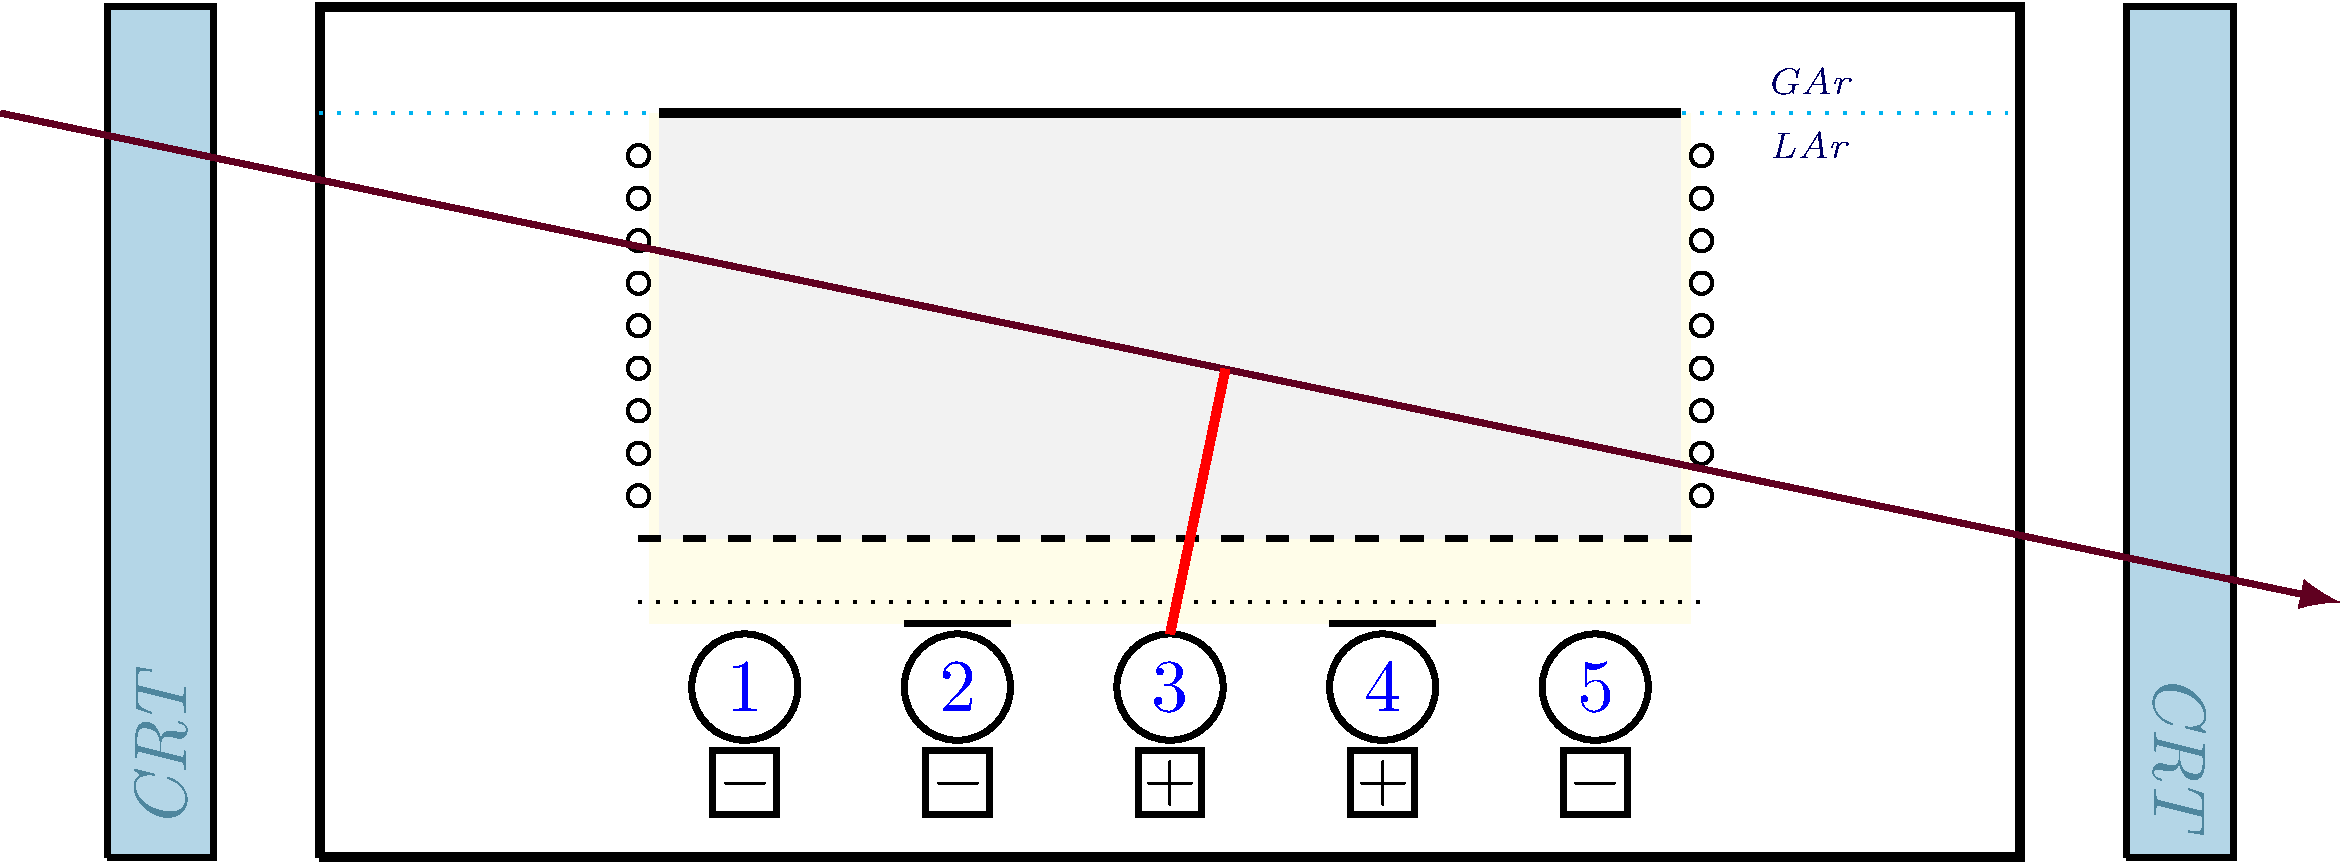
\includegraphics[width=0.75\textwidth]{graphics/dppd_7_2_v2}
\end{dunefigure}

From the \dword{pds} point of view, the \dword{wa105} operation lasted several months, as light has been collected during cool down, filling and commissioning stages of the demonstrator.
The \dword{pds} had shown very stable performance during all this period. 
In Fig.~\ref{fig:pd-pds-311-ped}, the  pedestal mean and RMS are shown for one positive and one negative base \dword{pmt} as a function of time, for \num{5} months of operation. 

\begin{dunefigure}[\dword{wa105} \dwords{pmt} mean pedestal and RMS]{fig:pd-pds-311-ped}{Pedestal mean (top) and RMS (bottom) for one negative base \dword{pmt} (black) and one positive base \dword{pmt} (red) in between July and December 2017 during the operation of \dword{wa105}.}
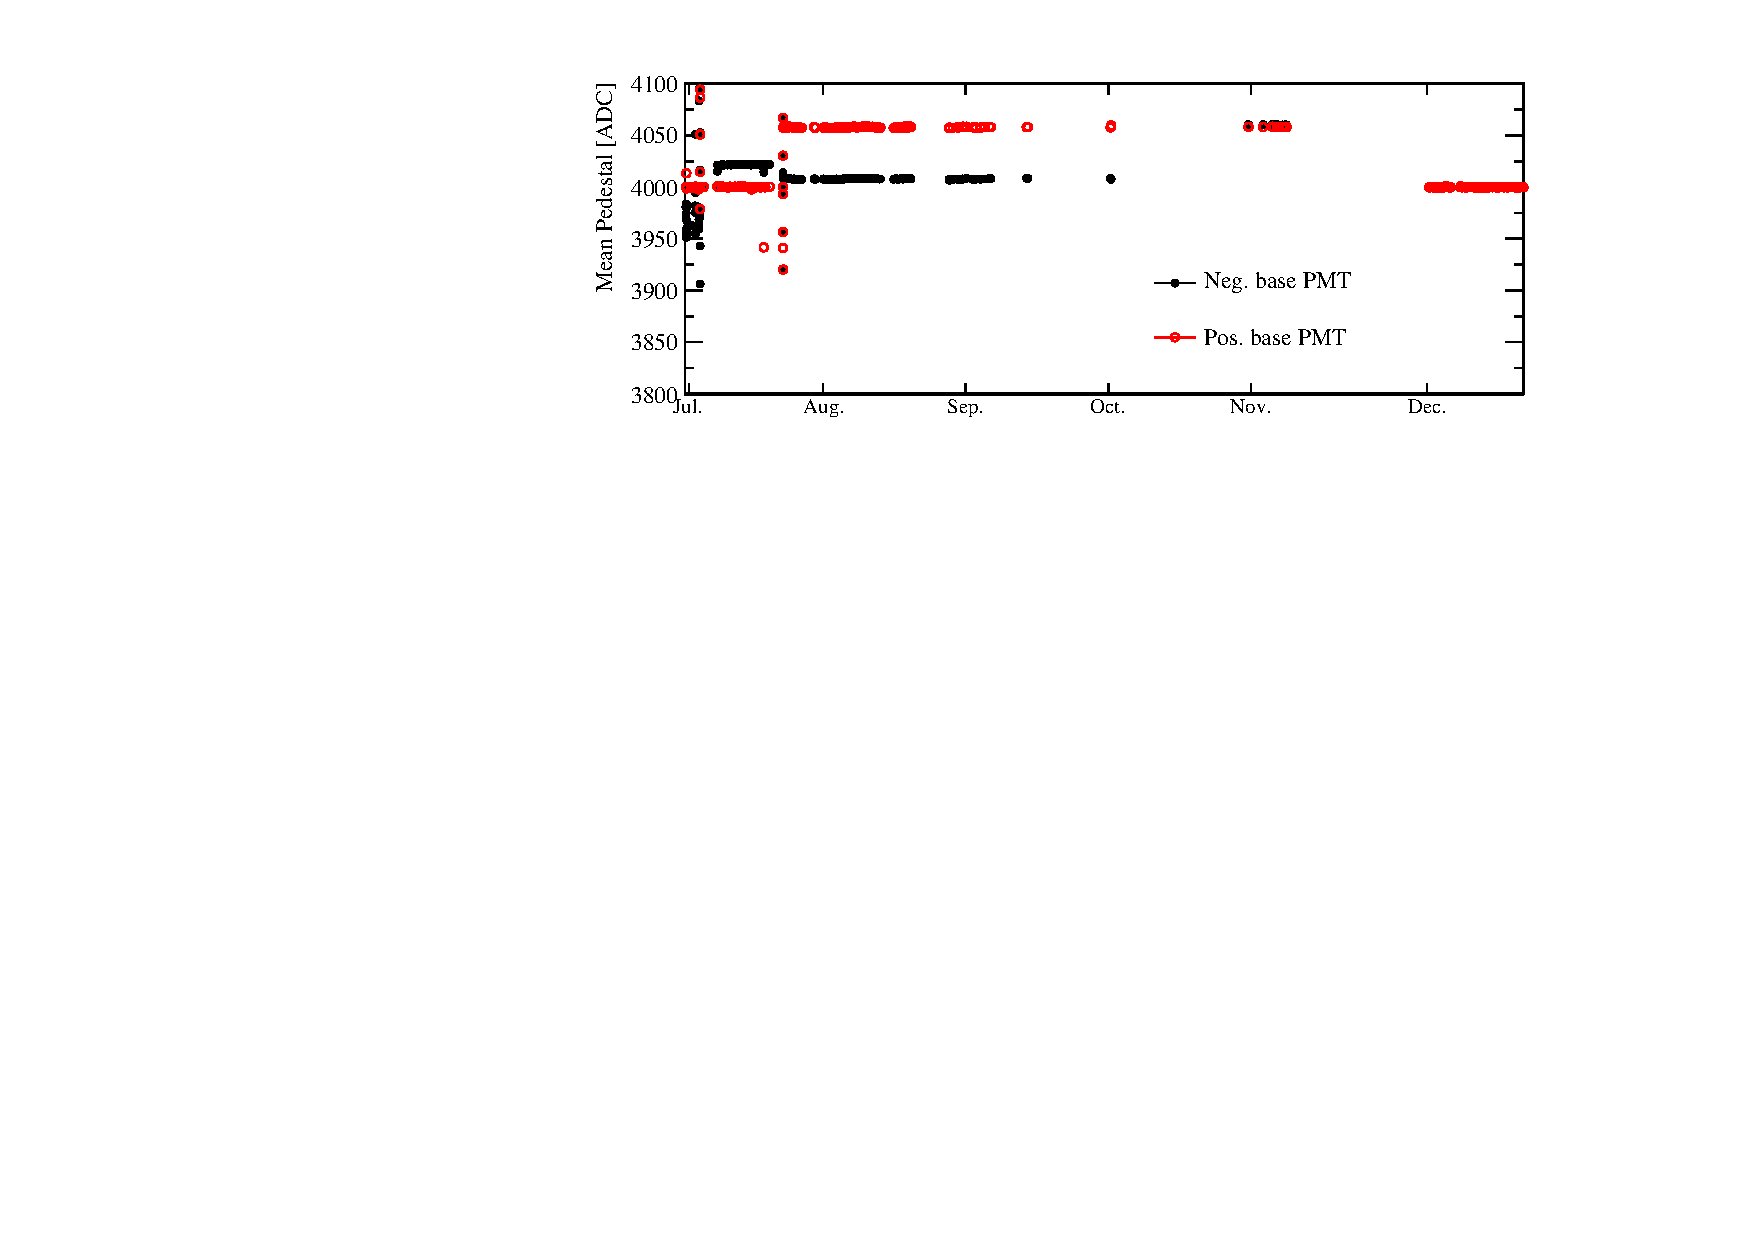
\includegraphics[width=0.9\textwidth]{graphics/dppd_311_pedestal.pdf}\\
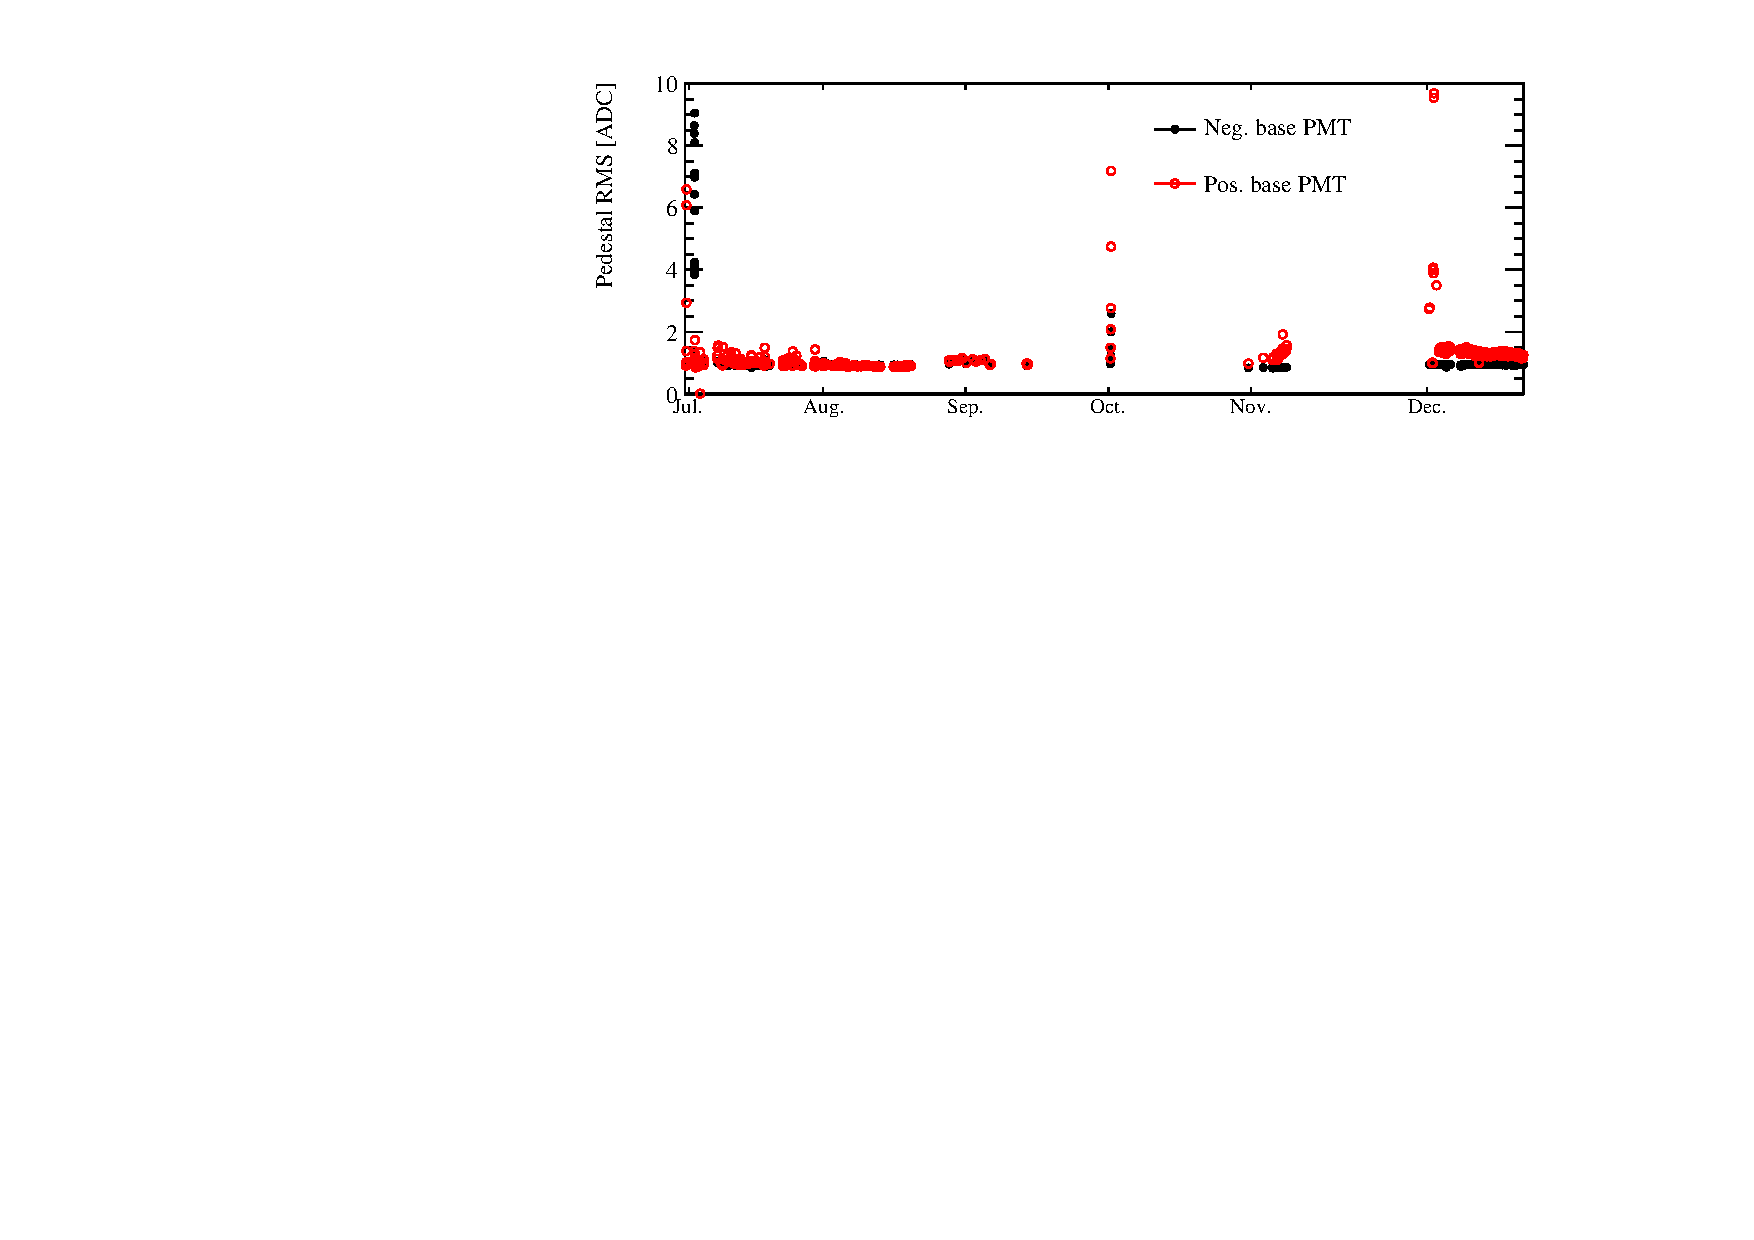
\includegraphics[width=0.9\textwidth]{graphics/dppd_311_pedestal_rms.pdf}
\end{dunefigure}

In Fig.~\ref{fig:pd-pds-311-LAr-GAr}, the average waveforms for \dword{pmt} 5 in gas and liquid argon with no drift field are presented. These waveforms are fitted with a gaussian -- to describe the response function -- convoluted with a sum of three exponentials -- for the description of the fast, slow and intermediate components. 
The extracted values agree with the literature, although the lifetime of the fast component has been fixed at \SI{6}{ns} in the fitting procedure.


\begin{dunefigure}[GAr and LAr scintillation profile in \dword{wa105}]{fig:pd-pds-311-LAr-GAr}{Scintillation time profile in the absence of drift field recorded in GAr (left) and LAr (right) in black. In red, the fit performed with a sum of 3 exponential (describing the fast, intermediate and slow components - all shown in dotted blue lines) convoluted with a gaussian to take into account the response function of the \dword{pmt}. The extracted lifetimes are shown in the figure.}
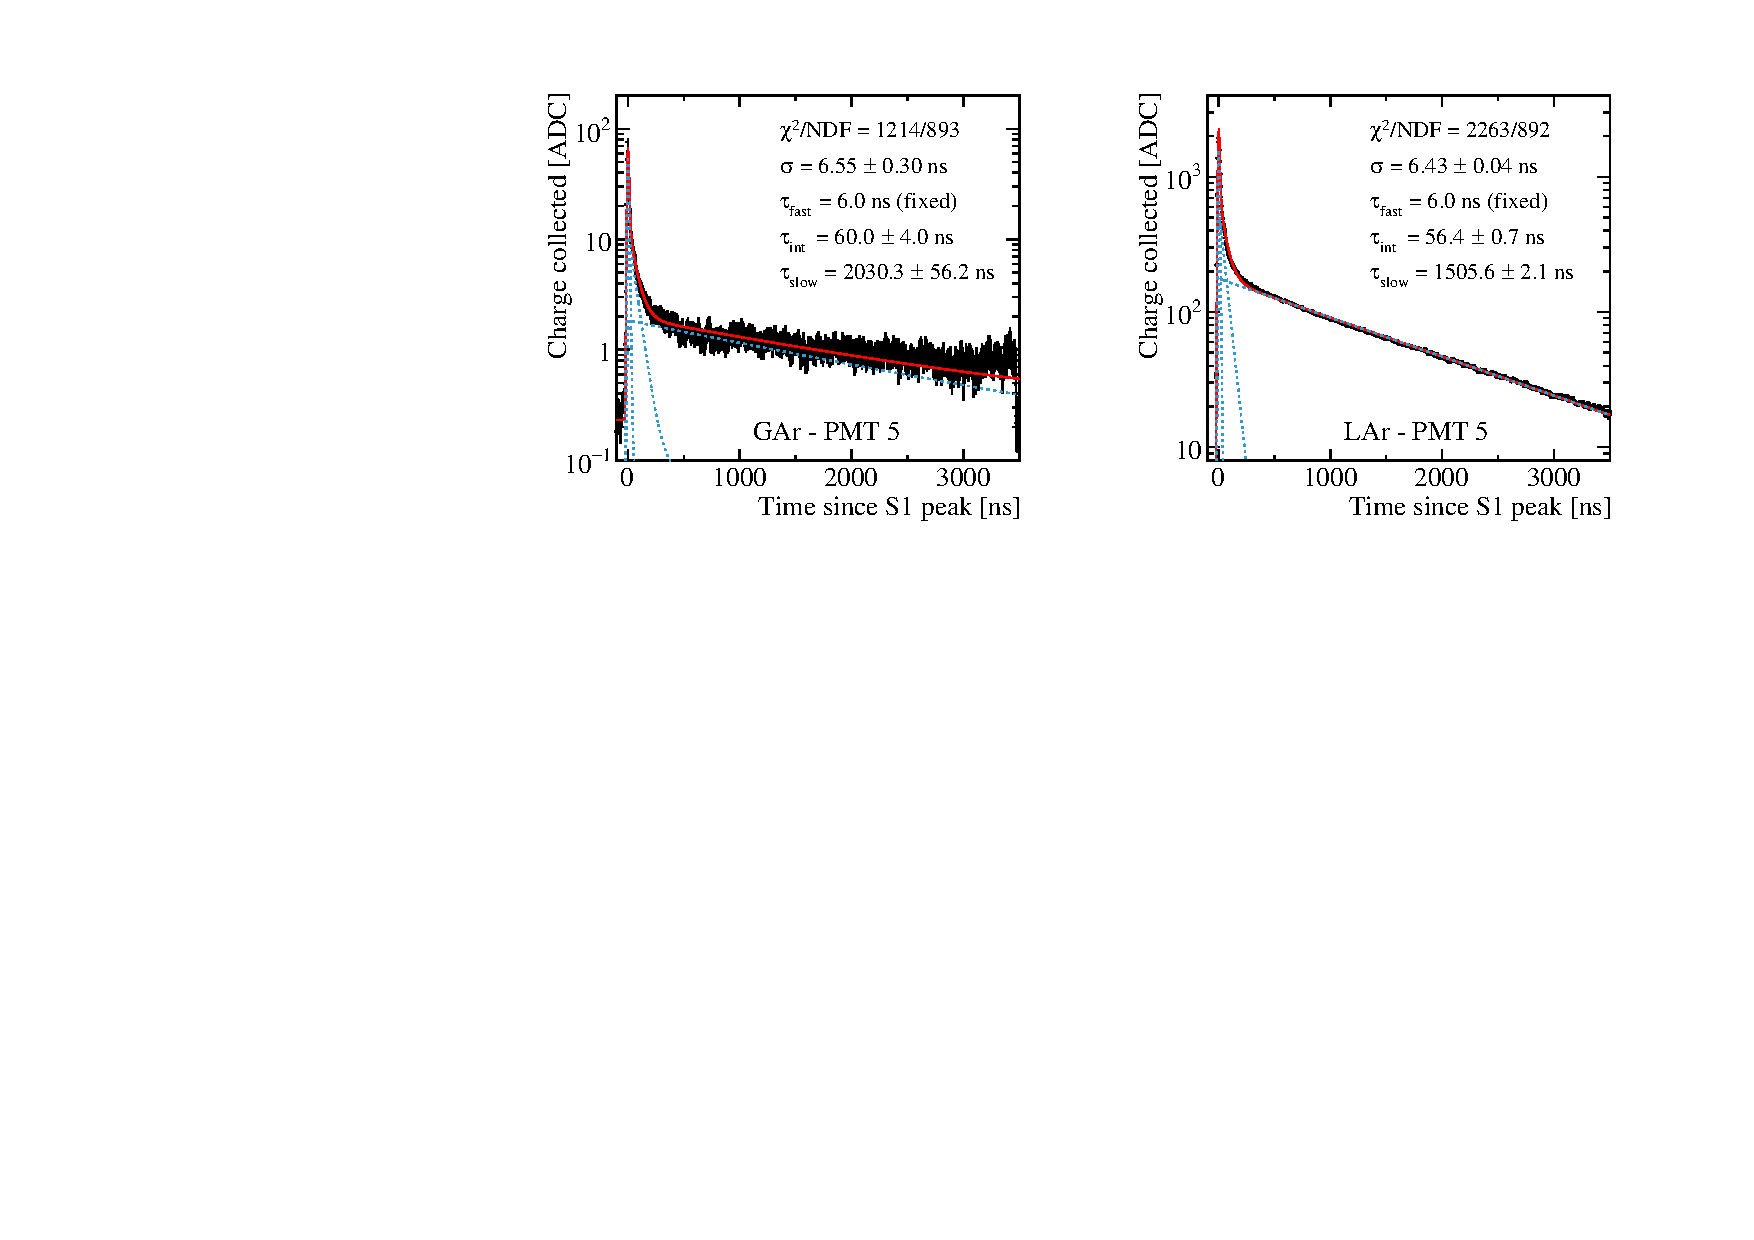
\includegraphics[width=0.85\textwidth]{graphics/dppd_311_lar_gar_fit.pdf}
\end{dunefigure}

It has been shown in many studies that $\tau_{slow}$, the slow component (Sec.~\ref{sec:dp-pds-overview_scintillation}), is very sensitive to the amount of impurities in the liquid.
In order to monitor the purity of the liquid argon as a function of time, the same fit has been performed on several runs taken with similar conditions. 
In Fig.~\ref{fig:pd-pds-311-purity}, the evolution of $\tau_{slow}$ for \SI{15}{days} of operation is presented.
The results exhibit a very stable amount of impurities, which is in agreement with the stability of the electron lifetime measured using the charge collection.

\begin{dunefigure}[Evolution of $\tau_{slow}$ as a function of time in \dword{wa105}]{fig:pd-pds-311-purity}{Evolution of $\tau_{slow}$ over \num{15} days of operation of the \dword{wa105}. The points are the averages over the values extracted from the fits to the waveforms of the \num{3} negative base \dwords{pmt} for runs taken with no drift field. Preliminary results.}
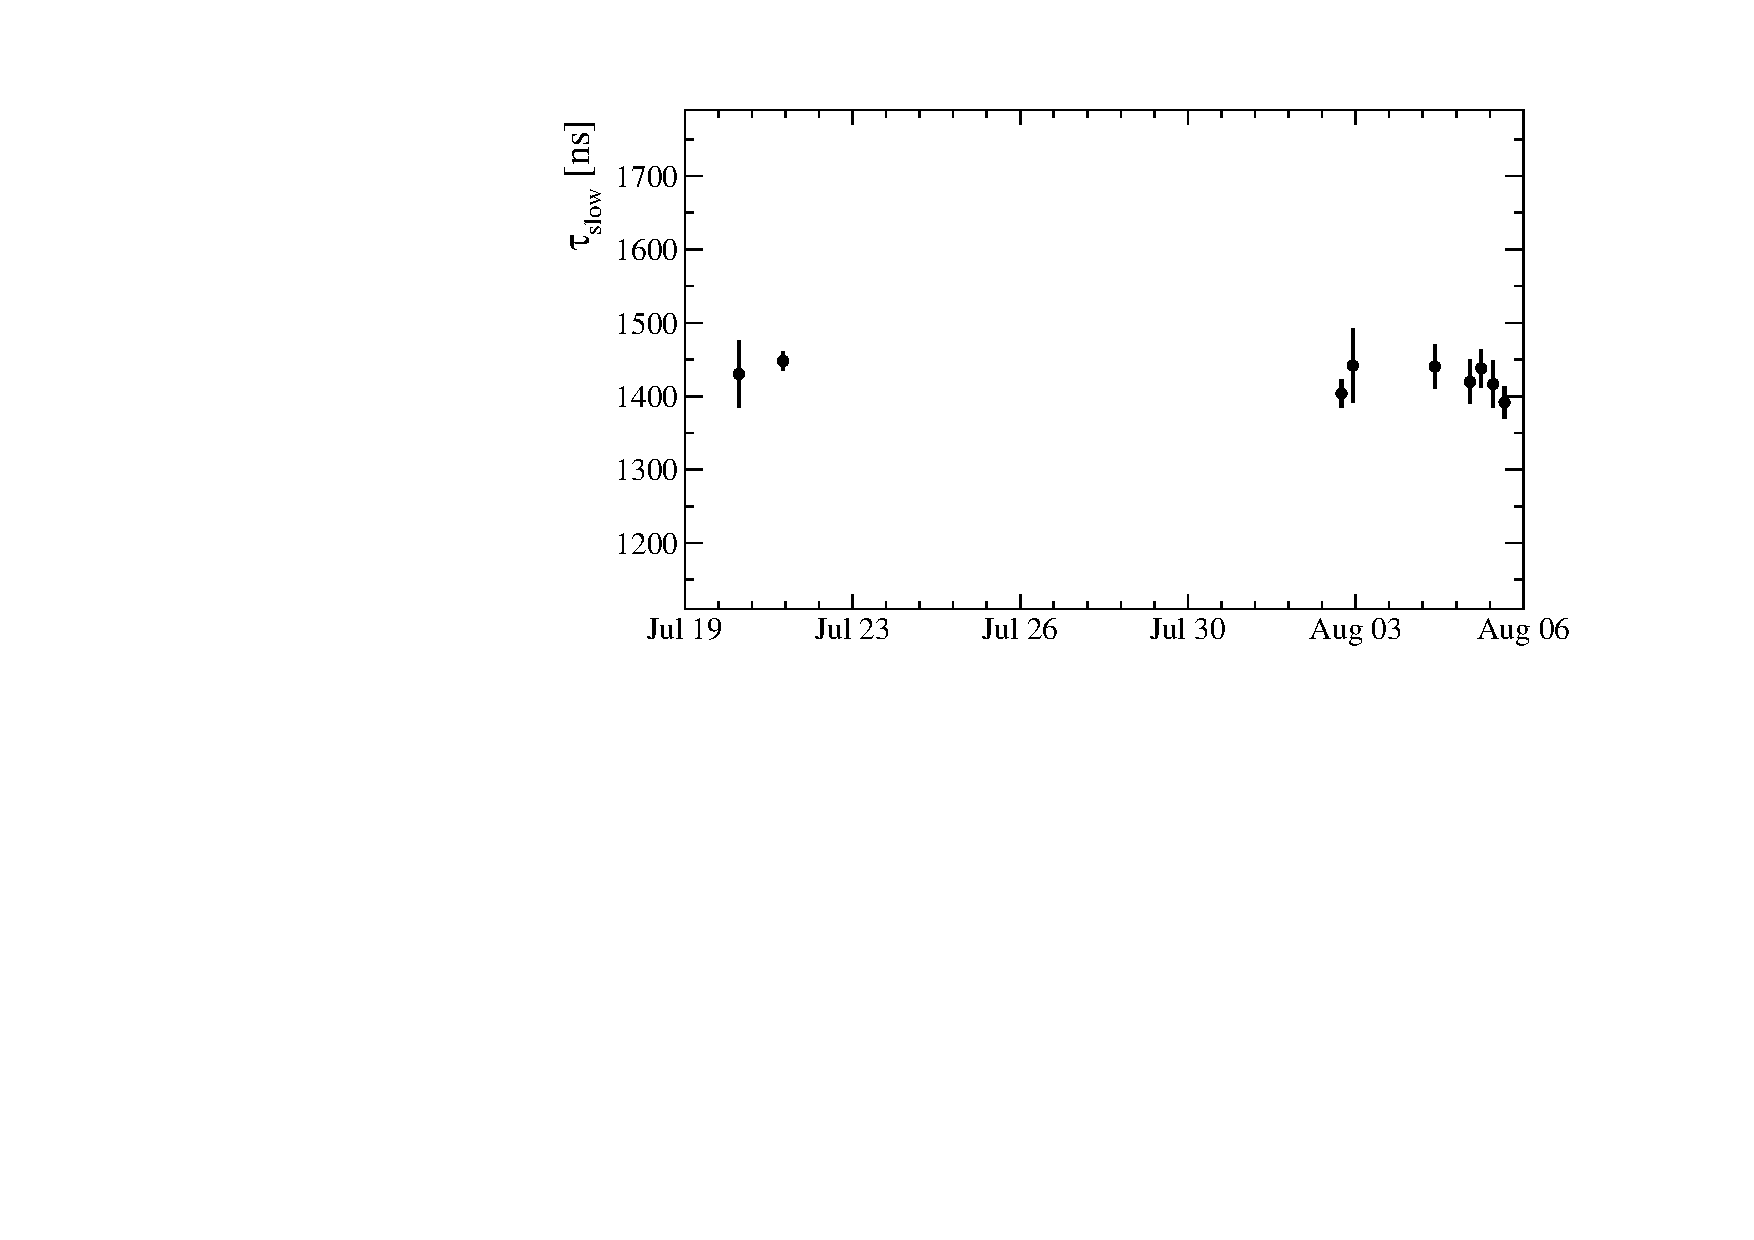
\includegraphics[width=0.8\textwidth]{graphics/dppd_311_purity.pdf}
\end{dunefigure}

The S2 light has also been recorded, with dedicated runs using a \SI{1}{ms} recording time window.
In Fig.~\ref{fig:pd-pds-311-S2}, the average waveforms are presented from runs taken with a drift field of \SI{0.5}{kV/cm} and an extraction field of \SI{2}{kV/cm} (\SI{3}{kV/cm}) in liquid (gas). In the figure, one run has no amplification field, the other have the \dwords{lem} polarized to provide an amplification field of \SI{25.5}{kV/cm}. 
One can clearly see the effect of the \dwords{lem} on the amount of S2 light generated. 
The S2 light extends for about \SI{600}{$\mu$s} after the emission of the prompt signal, which is in agreement with the electron drift time over \SI{1}{m} at such drift field.

\begin{dunefigure}[S2 light at different amplification field in \dword{wa105}.]{fig:pd-pds-311-S2}{Average waveforms of negative based \dwords{pmt} in a \SI{1}{ms} window. Both runs were taken with a drift field of \SI{0.5}{kV/cm} and an extraction field of \SI{3}{kV/cm} in gas. The S2 light extends for about \SI{600}{$\mu$s}, as expected.}
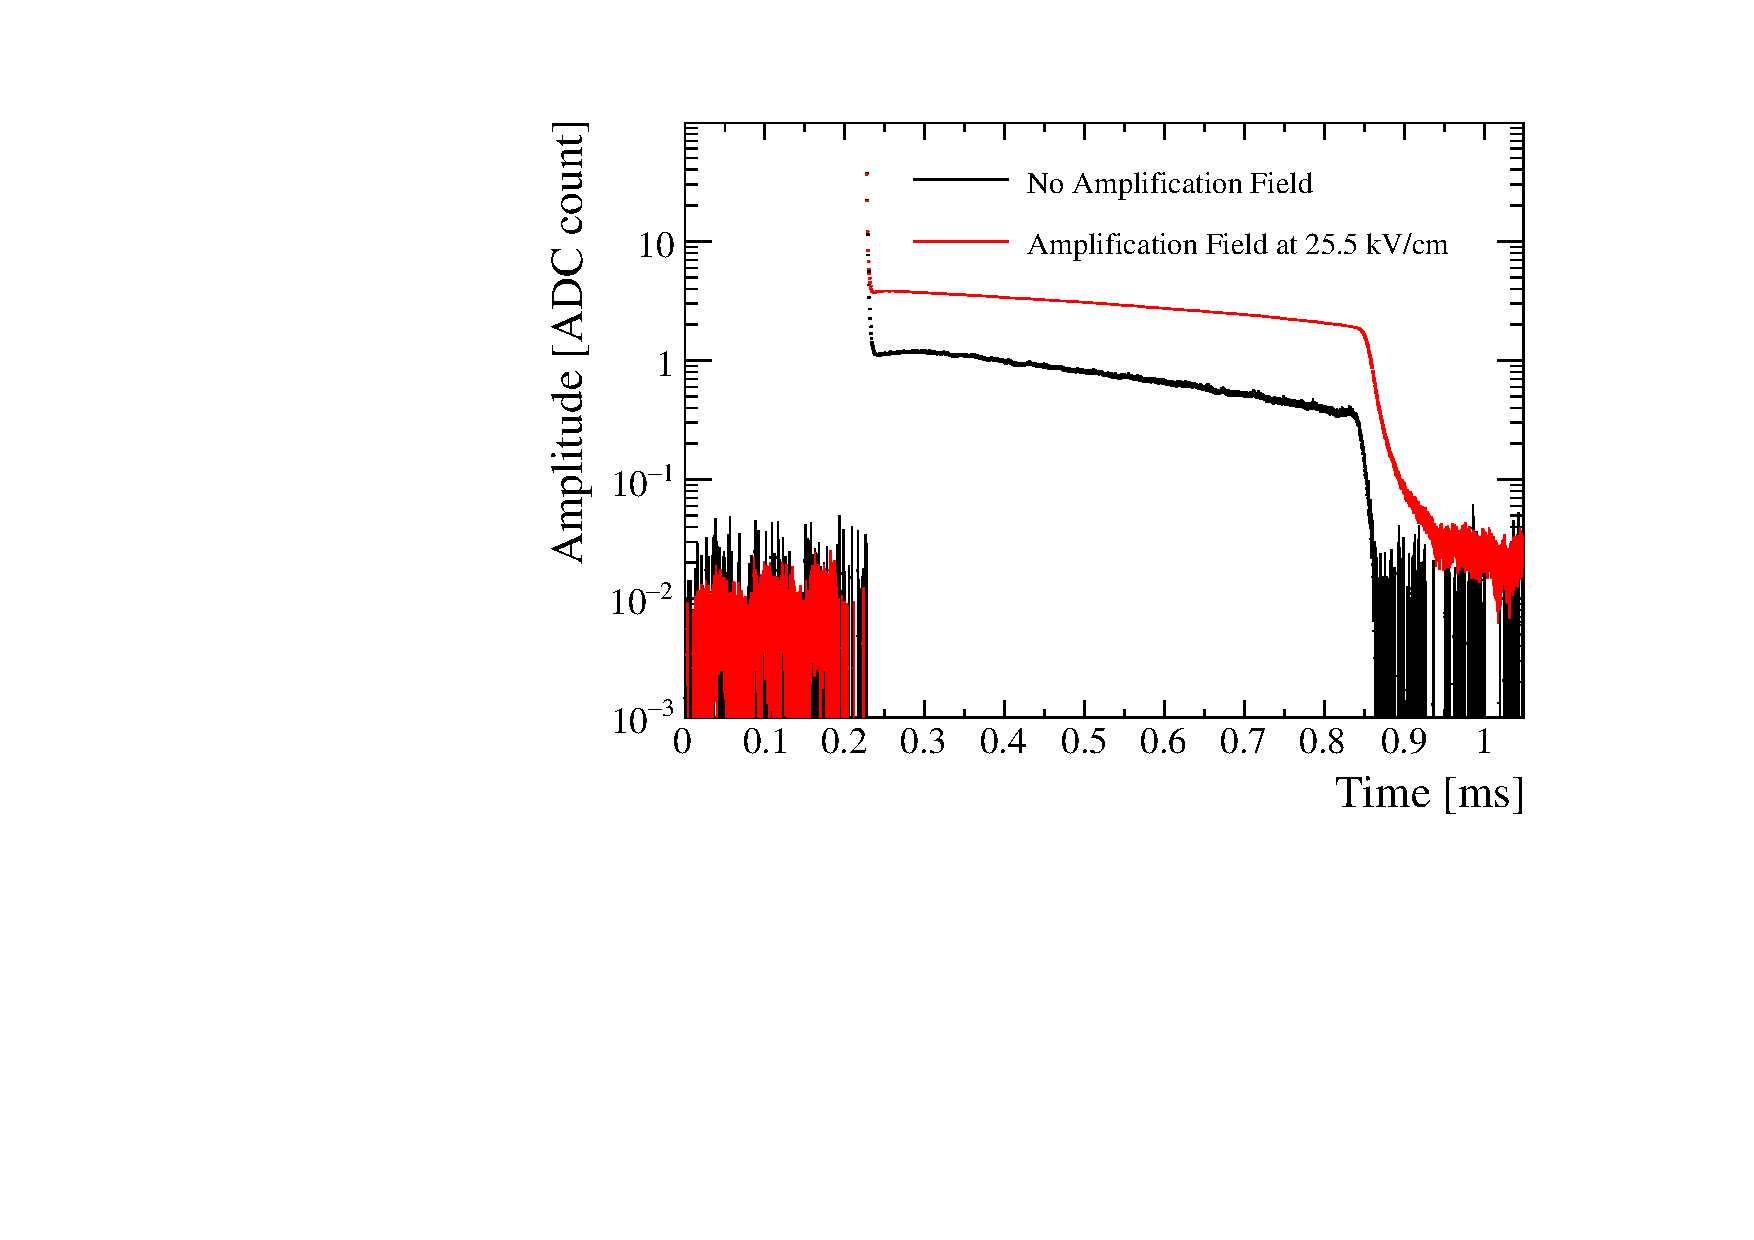
\includegraphics[width=0.8\textwidth]{graphics/dppd_311_S2_extraction.pdf}
\end{dunefigure}
Using data taken at null field in CRT triggering mode, a selection of muon-like tracks is performed. It is further required that the tracks cross the active volume for distances longer than \SI{3.1}{\m}. 
The S1 charge collected by each \dword{pmt} is calculated by integrating the ADC values in a \SI{1}{\us} window starting from the S1 peak, and this charge value is then converted into the number of detected photoelectrons (PEs) using the calibrated \dword{pmt} gains given in Table~\ref{tab:dp-pds-311conf}.

In the simulation, \SI{4}{\GeV} muons are generated from one CRT panel to the other with data-driven kinematics. The number of PEs collected by each \dword{pmt} is generated according to the light maps. A selection on the minimum amount of light recorded by all \dwords{pmt} in order to suppress spurious triggers is used in the data analysis and does not apply to the case of MC. Additionally, the requirement that the \dword{pmt} signal does not saturate the readout is implemented only for the data analysis and not MC. A comparison of the number of PEs collected in data and in MC is presented in Fig.~\ref{fig:dp-pds-311charge}. The result shows a good agreement between data and MC.

In the \dword{wa105}, the \dword{pmt} gain was adjusted such that S1 and S2 light could be seen, and to increase the trigger rate while minimizing the \dword{pmt} ADC saturation. 
In \dune \dual, the situation will be different as the volume is much larger and part of the triggering modes will be independent from the \dwords{pmt}. 
Hence the \dword{pmt} gain will be adjusted accordingly and the events saturating the ADC should not be as problematic as it could be in \dword{wa105}.
%\fixme{Give more details about why \dword{pmt} saturation in \dword{wa105}, and why this is not worrisome in \dpmod?}

\begin{dunefigure}[Charge Collected in \dword{wa105} vs MC]{fig:dp-pds-311charge}{ Charge collected by the \dwords{pmt} in a \SI{1}{\us} window containing the S1 peak for muon-like tracks triggered by the CRT panels. The data is shown with black and the simulation with red. The distributions are normalized to unity for clarity. Preliminary results.}
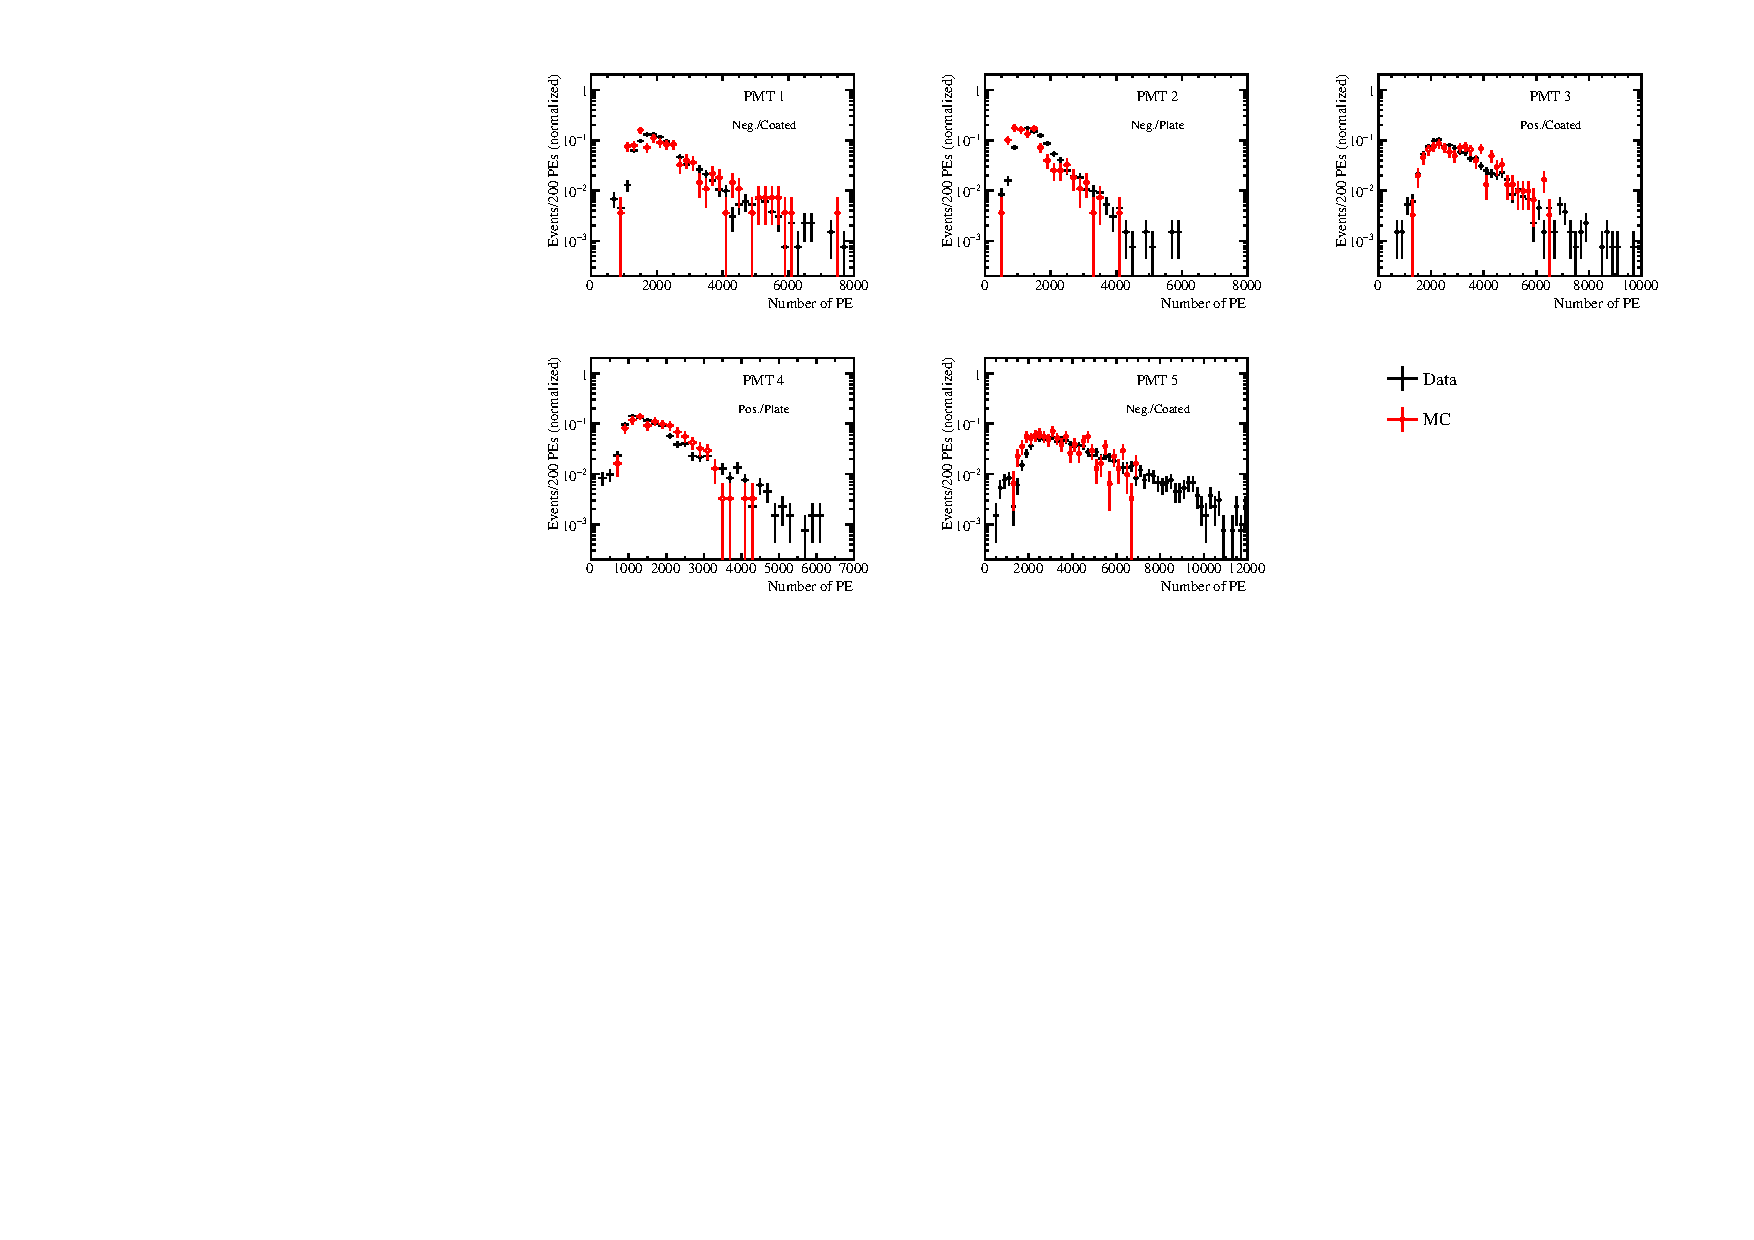
\includegraphics[width=0.95\textwidth]{graphics/dppd_311_charge_mc_v2.pdf}
\end{dunefigure}

\begin{dunefigure}[Charge Collected vs track-PMT shortest distance]{fig:dp-pds-311profile}{Profile histograms of charge collected as a function of the track-PMT shortest distance. The data is in black, the simulation in red. Preliminary results.}
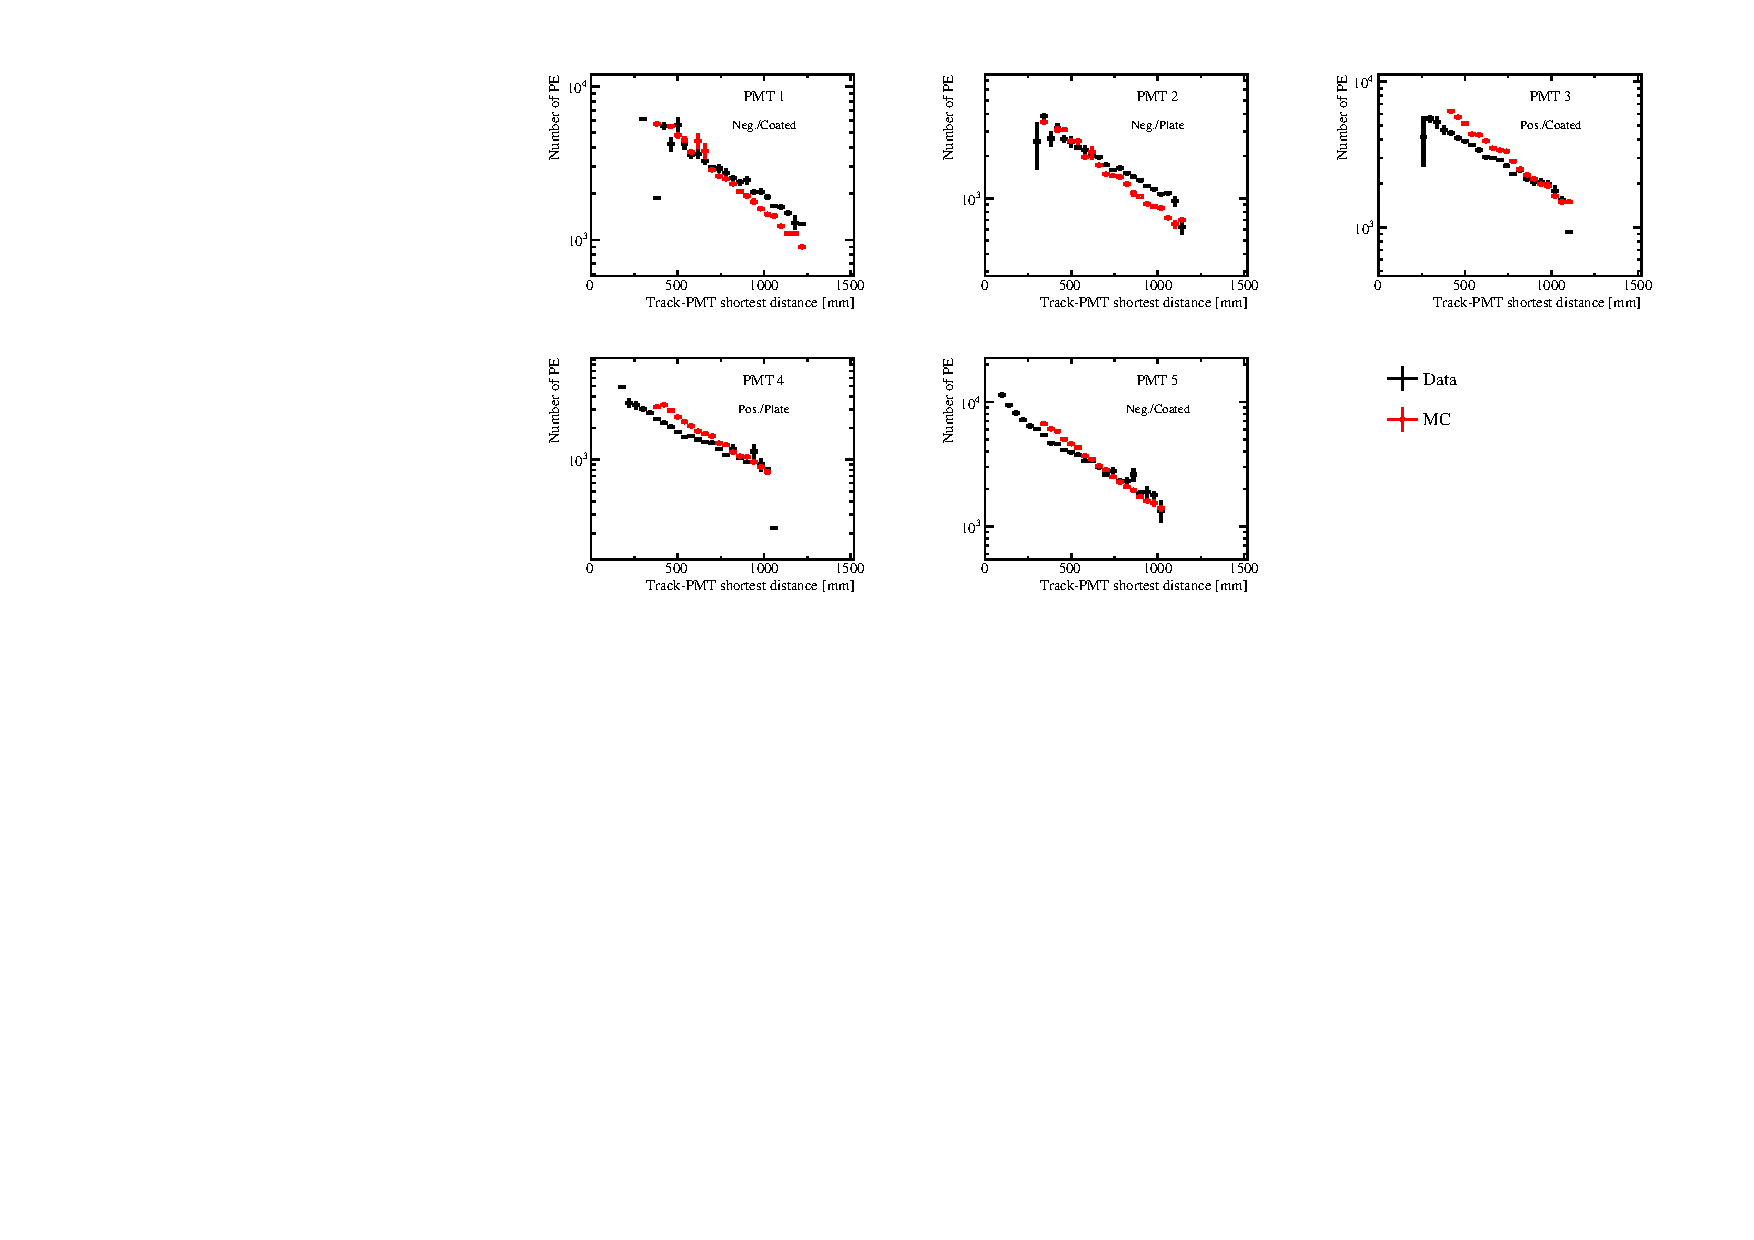
\includegraphics[width=0.95\textwidth]{graphics/dppd_311_charge_dist_mc.pdf}
\end{dunefigure}

%\fixme{This is rather distance vs charge. Is it possible to swap the x and y axis and reproduce the plots?}

The amount of PEs collected per \dword{pmt} depends strongly on the shortest track-\dword{pmt} distance. Many factors can affect the amount of charge collected, the dominant one being the scattering length, also known as the Rayleigh scattering length. This quantity is still subject to debate among the \dword{lar} community as its measurement is fairly complicated. Current estimates of the scattering length range from \SI{20}{\cm} to \SI{1}{\m}.
In the \dword{wa105} simulation, the scattering length was set to L$_{ray}$ = \SI{55}{\cm}.
Figure~\ref{fig:dp-pds-311profile} shows the charge collected as a function of the shortest track-\dword{pmt} distance in the form of profile histograms. The overall trend is very similar for data and MC, also across all the \dwords{pmt}. However, the profile histogram slopes indicate that the assumed scattering length in MC could be better tuned to reproduce the data, e.g. towards larger values of the Rayleigh scattering length.

%%%%%%%%%%%%%%%%%%%%%%%%%%%%%%%%%%%%%%%%%%%%%%%%%%%%%%%%%%%%%%%%%%%%

\subsection{Preliminary (or Prospects for) ProtoDUNE-DP Light Data Results}

\fixme{Add lessons learned from \dword{pddp} installation and commissioning here?}